\documentclass{beamer}

\usepackage{gensymb}
\usepackage[utf8]{inputenc}
\DeclareUnicodeCharacter{00A0}{ }%Permet d'éviter certains conflits de caractères invisibles
\usepackage{amssymb}            % Principaux symboles
%\usepackage{fontspec}
%\usepackage{xunicode}
%\usepackage{xltxtra}
\usepackage[frenchb]{babel}
%\defaultfontfeatures{Scale=MatchLowercase}
%\setmainfont[Mapping=tex-text,Ligatures={Common, Historical}]{Linux Libertine O}
%\setsansfont[Mapping=tex-text]{Linux Biolinum O}
%\setmonofont[Scale=0.75]{DejaVu Sans Mono}

%% Packages pour le texte
%\usepackage[misc,geometry]{ifsym}	% Police numéros battons
\usepackage{pifont}		% Police \ding
\usepackage{eurosym}		% Symbole de l'euro
\usepackage{soul}		% Souligner
\usepackage{enumerate}		% Listes
\usepackage{verbatim}		% Codes source
\usepackage{moreverb}		%	et listings
\usepackage{textcomp}
\usepackage{multicol}

%% Packages pour les tableaux
\usepackage{array}		% Outils supplémentaires
\usepackage{multirow}		% Colonnes multiples
\usepackage{tabularx}		% Largeur totale donnée
\usepackage{longtable}		% Sur plusieurs pages

%% Les packages pour les dessins
\usepackage{graphicx}		% Insertion de figures
%\usepackage{picins}		% Dans un paragraphe
\usepackage{epic}		% Capacités graphiques
\usepackage{eepic}		% 	étendues
\usepackage{afterpage}		% Voir page 69
\usepackage{rotating}		% Tourner du texte
\usepackage{caption}		% Légendes
% \addto\captionsfrench{\def\figurename{}}

%% Packages pour les maths
\usepackage{amsmath}		% Commandes essentielles
\usepackage{amssymb}		% Principaux symboles
\usepackage{mathrsfs}		% Police calligraphique
\usepackage{theorem}		% Théorèmes
%\usepackage{tikz}		% Courbes
\usepackage{esvect}            % Vecteurs
%\usetikzlibrary{shapes,arrows,shadows}
\usepackage{pgf}
%\usetikzlibrary{arrows}
% Packages pour la physique
%\usepackage{sistyle}		% Unités
\usepackage[version=3]{mhchem}	% Formules chimiques
\usepackage{etex}
%\usepackage{m-pictex,m-ch-en}

%\usepackage{media9}
\usepackage{multimedia}		% Vidéos dans la présentation
%\usepackage{movie15}

%Ajout d'images de fond:
\usepackage{eso-pic}
\usepackage{wallpaper}

\usepackage{ccicons}		% Licence creativecommons

%\SIdecimalsign{,}


\AtBeginSection[]
{
  \begin{frame}
    \frametitle{Sommaire}
    \begin{multicols}{2}
      {\small
				\setcounter{tocdepth}{2}
        \tableofcontents[currentsection, hideothersubsections]}
    \end{multicols}
  \end{frame}
}

\usetheme{Warsaw}

\usepackage{listings}
\usepackage[babel=true]{csquotes}
\lstset{language=Python, tabsize=2, breaklines=true, showstringspaces=false}

\definecolor{RedT}{rgb}{1, .7, .7}
\definecolor{GreenT}{rgb}{.7, 1, .7}
\definecolor{OrangeT}{rgb}{1, 1, .7}

\useoutertheme{infolines}
\setbeamersize{text margin left=1cm,text margin right=1cm}

\title{Rapport de projet de SI}
\subtitle{Tropodrone}
\author{Gueydan Noé, Manceau Thibaut, Gros Alexis, Porteries Tristan}

\begin{document}

\begin{frame}
  \titlepage
\end{frame}

\begin{frame}
    \frametitle{Sommaire}
    \begin{multicols}{2}
      {
		\setcounter{tocdepth}{1}
        \tableofcontents
      }
    \end{multicols}
\end{frame}

\section{Courte présentation}

\subsection{But du projet}
\begin{frame}{But du projet}
 Créer une structure composée de ballons contenant un gaz plus léger que l’air qui soutient une partie ou la totalité du poids d'un drone.
\end{frame}


\subsection{Objectifs}
\begin{frame}{Objectifs}
 Augmenter l’autonomie, la sécurité et les possibilités d’un drone de petite taille
\end{frame}


\subsection{Contraintes imposées au projet}
\begin{frame}{Contraintes imposées au projet}
  \begin{itemize}
    \item être simple d’utilisation, garder la manœuvrabilité du drone au possible, voler le plus longtemps possible~;
    \item consommer le moins d’énergie possible, ne pas présenter de danger pour le public et économiser le gaz et les matériaux de fabrication~;
    \item le modèle du drone imposé~;
    \item rayon d’action de minimum 15 mètres~;
    \item ballon de type dirigeable.
  \end{itemize}
\end{frame}

\subsection{Contraintes légales supplémentaires}
\begin{frame}{Contraintes légales supplémentaires}
  \begin{itemize}
    \item 1~: Le drone \\
	    catégorie A~: limitations non contraignantes~;
    \item 2~: Le ballon \\
	    catégorie « Léger » \\
	    la ficelle supportant la charge doit casser au dessus de 23 kg.
 \end{itemize}
\end{frame}


\section{Drone}

\subsection{Modèle}

\begin{frame}
  \begin{multicols}{2}
    Drone XCSOURCE~: \\
    \begin{itemize}
      \item 290 mm diagonale~;
      \item 190 mm longueur~;
      \item 70 mm hauteur~;
      \item moteur EMAX MT2204 2300KV Brushless Motor~;
      \item Accu Lipo Gens Ace 2200Mah 11.1V 25C 3S~;
      \item 450 g.
    \end{itemize}
    \newpage
    \begin{center}
      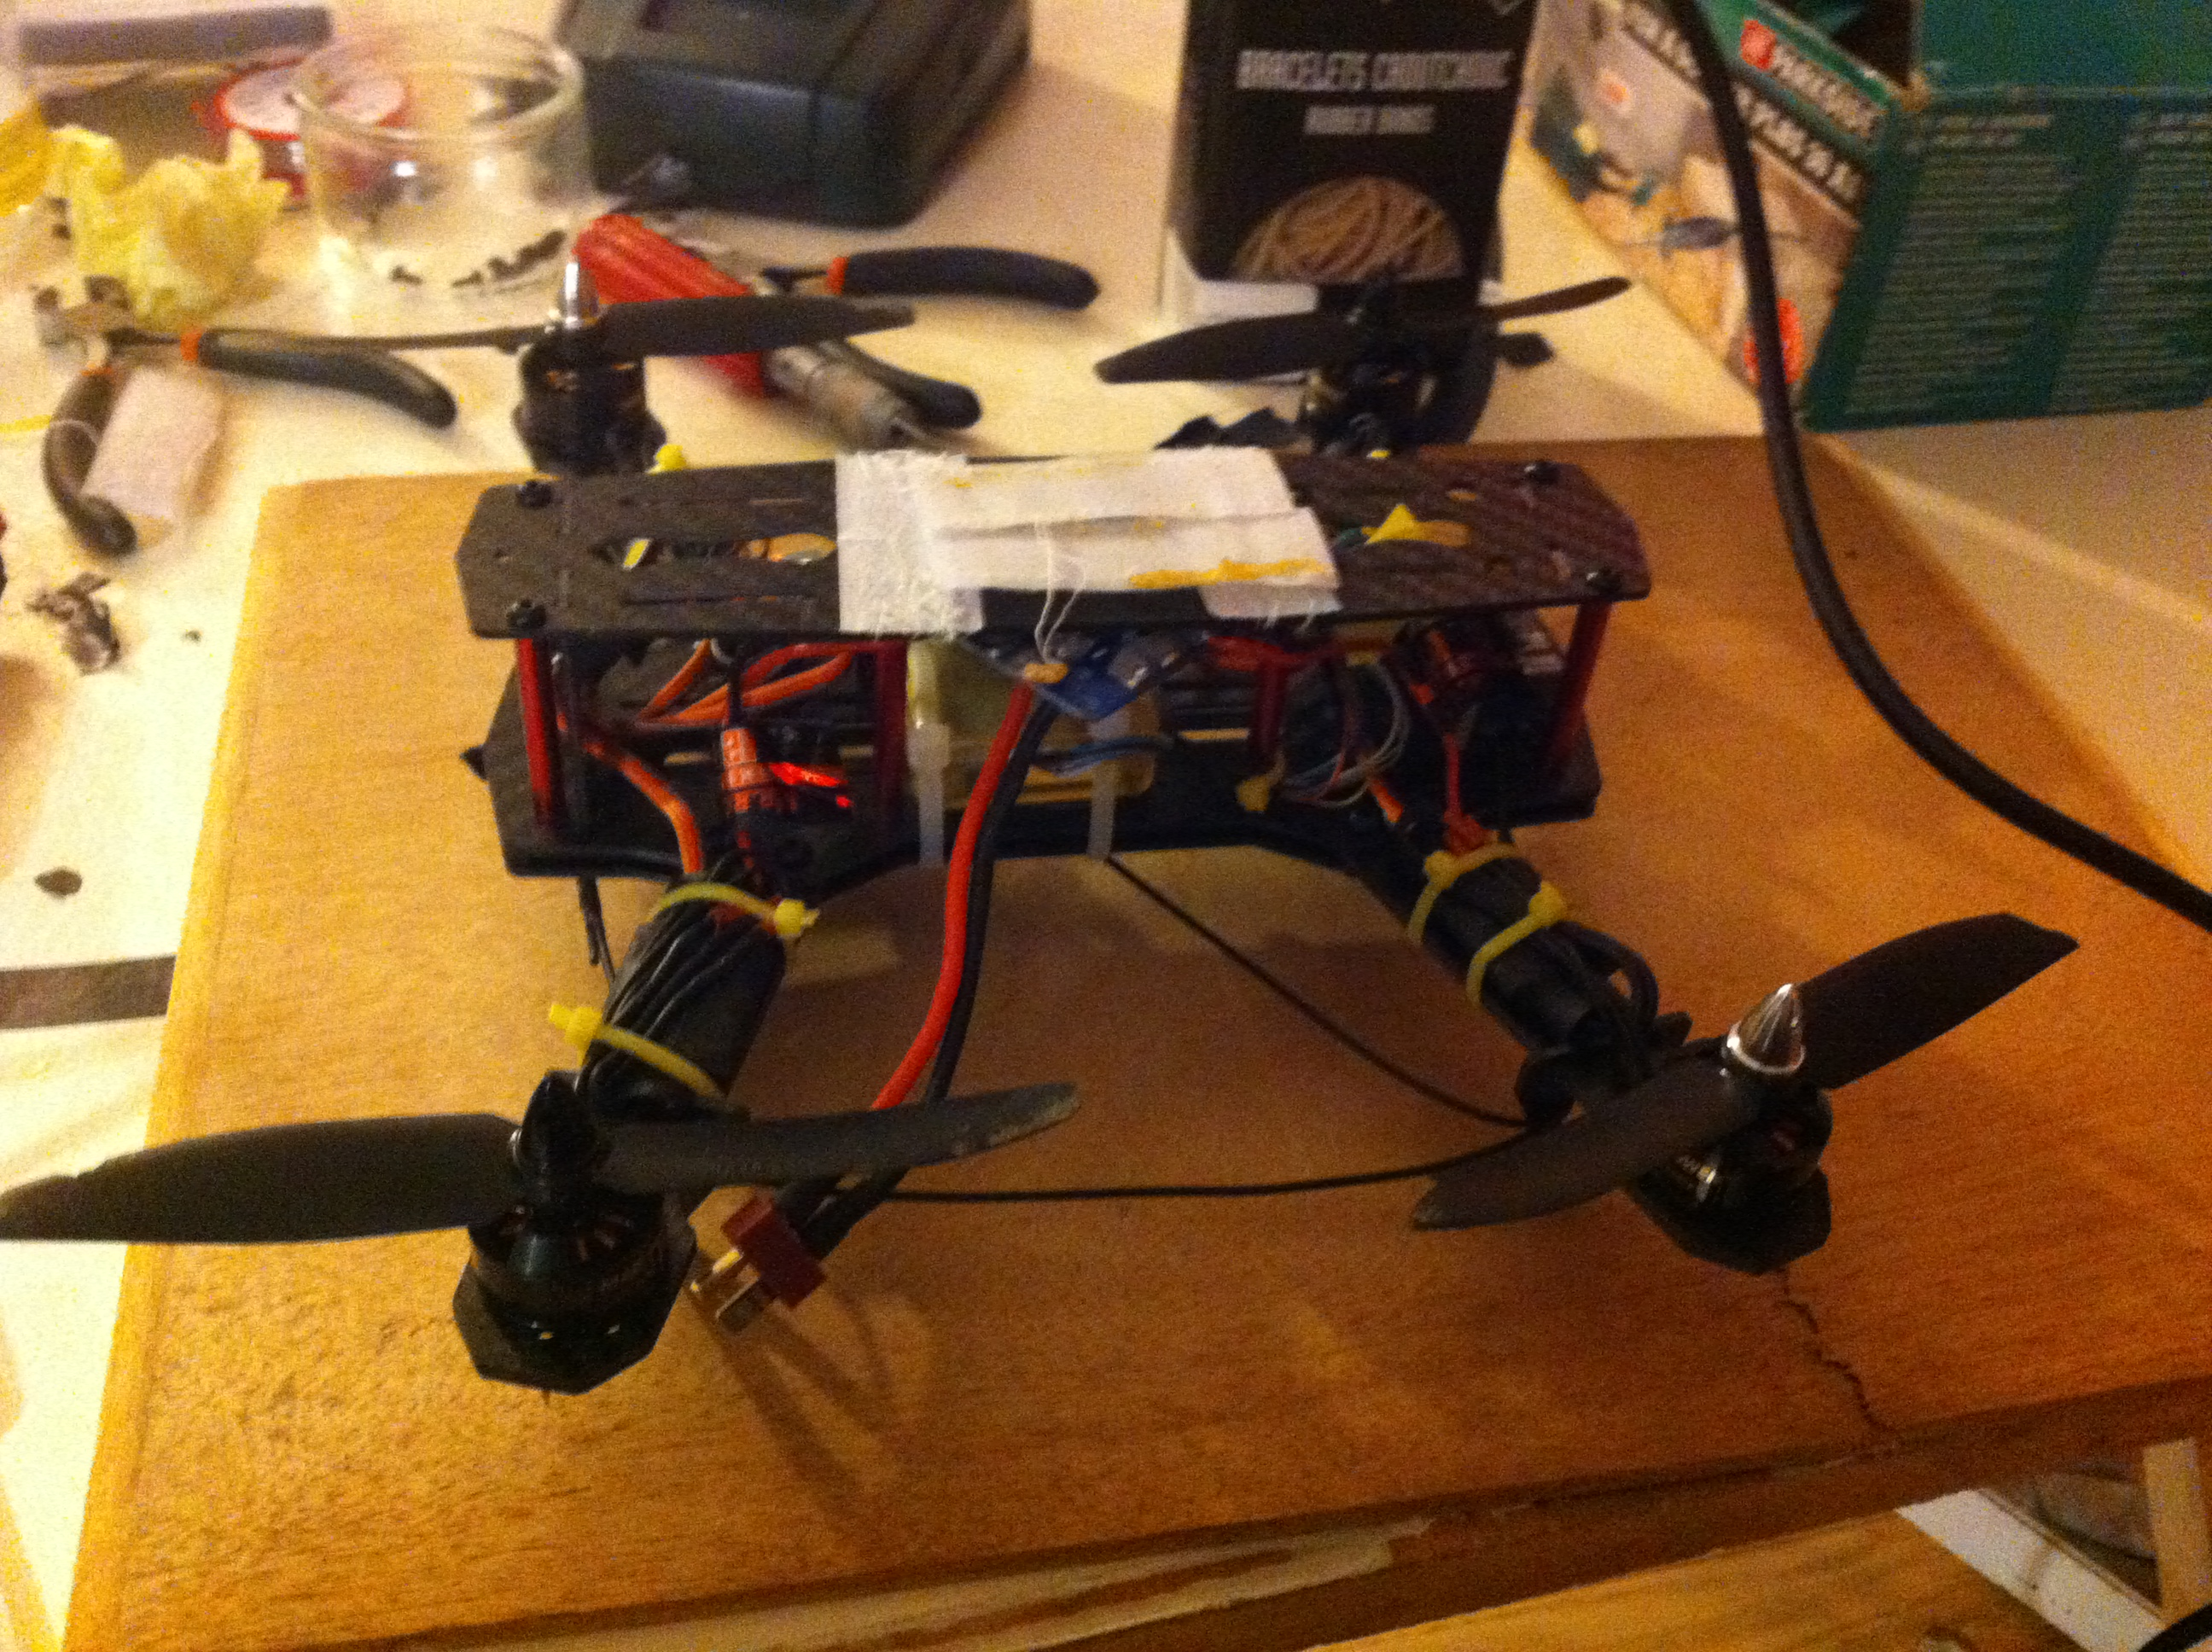
\includegraphics[width=6cm]{../Images/drone.JPG}
    \end{center}
    \captionof{figure}{Drone XCSOURCE.}
  \end{multicols}
\end{frame}




\section{Calculs d'élévation}

\subsection{Poussé d'Archimède}

\begin{frame}{Définition}
  \enquote{Tout corps plongé dans un fluide au repos, entièrement mouillé par celui-ci ou traversant sa surface libre, subit une force verticale, dirigée de bas en haut et opposée au poids du volume de fluide déplacé ; cette force est appelée poussée d'Archimède.}
  \bigbreak
  \begin{center}
    \boxed{\vv{Pa} = -M_F \times \vv{g}}
  \end{center}
  \begin{itemize}
    \item $\vv{Pa}$~: la poussé d'Archimède~;
    \item $M_F$~: la masse du fluide contenue dans le volume déplacé~;
    \item $\vv{g}$~: la valeur du champ de pesanteur.
  \end{itemize}
\end{frame}

\begin{frame}{Application aux ballons}
  Deux forces appliquées sur le ballon~: \\
  \begin{center}
    $\displaystyle{\vv{F_{ballon}} = \vv{P_{ballon}} + \vv{Pa_{ballon}}}$ \\
  \end{center}
  Si $P_{ballon} < Pa_{ballon}$ la force d'élévation est~:
  \begin{center}
    $\displaystyle{F_{ballon} = Pa_{ballon} - P_{ballon}}$ \\
  \end{center}
  Remarque~:\\
  \begin{center}
    $F_{ballon} < Pa_{ballon}$
  \end{center}
\end{frame}

\begin{frame}{Hydrogène et hélium}
	\begin{center}
		\begin{tabular}{|l|c|c|c|}
			\hline
			Gaz & Air & Hydrogène & Hélium \\
			\hline
			Masse Volumique $(kg.m^3)$ & 1.29 & 0.08988 & 0.1785 \\
			\hline
			Force d'élévation $(N.m^3)$ & 0 & 11.77 & 10.90 \\
			\hline
		\end{tabular}
	\end{center}
\end{frame}



\subsection{Dilatation des gaz}

\begin{frame}{Ballon chauffé}
	Combiner une montgolfière et un gaz plus léger.
	
	Réduire la masse volumique du gaz en le chauffant~: augmentation de la force d'élévation car moins de poids.
\end{frame}



\begin{frame}{Loi de Charles}
  \begin{center}
    \boxed{\displaystyle{\frac{V_1}{T_1} = \frac{V_2}{T_2} = f(P, n)}} \\
    $\displaystyle{V_3 = f(P, n) \times T_3}$
  \end{center}
  Avec~:
  \begin{itemize}
    \item $V_q$~: volume du gaz en $m^3$ à la température $T_q$ en K~;
    \item $P$~: pression du gaz en Pa~;
    \item $n$~: quantité de matière en mol~;
    \item $f(P, n)$~: rapport constant entre volume et température.
  \end{itemize}
\end{frame}

\begin{frame}{Application à l'hélium}
  Volume molaire de l'hélium~: $22.414\times 10^{-3} m^3.mol^{-1}$ à $273.25K$.
  \begin{center}
    $\displaystyle{f(P, n) = \frac{22.414\times 10^{-3}}{273.25} = 8.2\times 10^{-5} m^3.mol^{-1}.K^{-1}}$
  \end{center}
  Pour $T_{200} = 200 \degree C = 473.25 K$~:
  \begin{center}
    $\displaystyle{V_{T_{200}} = 8.2\times 10^{-5} * 473.25 = 38.811 \times 10^{-3}} m^3.mol^{-1}$
  \end{center}
  Augmentation du volume de $1.59$.
\end{frame}

\begin{frame}{Résultat de la poussé d'Archimède}
  \begin{center}
    $\displaystyle{F_{T_0} = Pa_{air} - P_{helium} = 10.90 N}$
    \bigbreak
    $\displaystyle{F_{T_{200}} = Pa_{air} - \frac{P_{helium}}{1.59} = 11.57 N}$ \\
  \end{center}
  Les résultats sont négligeables. $F < Pa_{air}$
\end{frame}


\section{Ballon}

\subsection{Modèle de ballon}

\begin{frame}{Contrainte des ballons}
	\begin{itemize}
		\item centre de gravité du drone et du ballon confondues~: pas de balancement~;
		\item ensemble de trois ballons répartis en triangle~;
		\item forme rigide~: contrôle de l'aérodynamisme.
	\end{itemize}
\end{frame}

\subsection{Contenance}

\begin{frame}{Bilan des masses et volumes}
	\begin{center}
		\begin{tabular}{|c|c|c|c|}
			\hline
			Élément & Drone & Ballon & Total (avec marge) \\
			\hline
			Masse (en g) & 450 & 250 & 750 \\
			\hline
		\end{tabular}

	\end{center}

  Volume d'hélium nécessaire~: $0.75 m^3$
  
  Volume des ballons~: $0.25 m^3$
\end{frame}

\subsection{Forme}

\begin{frame}{Contraintes de la forme des ballons}
  Les ballons sont formés d'un parallélépipède de longueur 1m avec deux pyramides d'angle $60\degree$. Orientation horizontale de $45\degree$ \\
  \begin{center}
    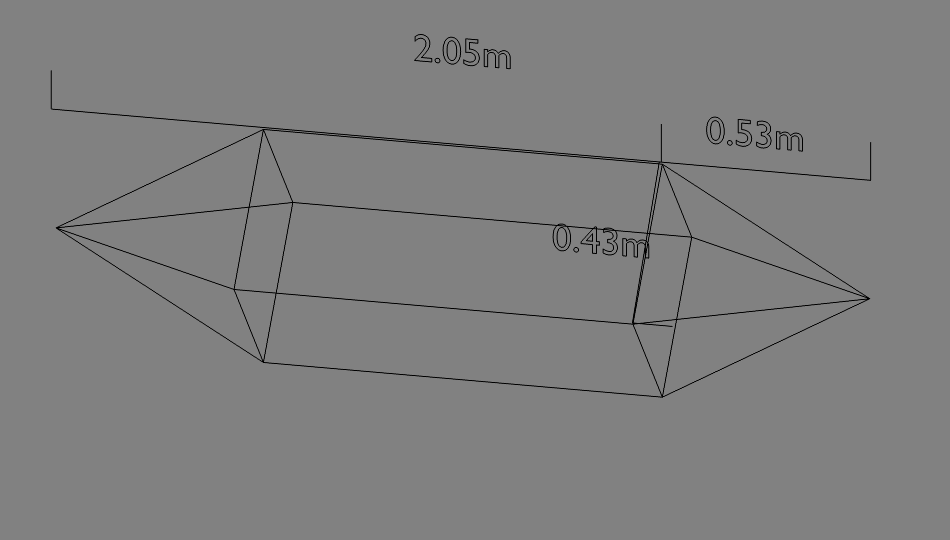
\includegraphics[width=7cm]{../Images/ballon.png}
    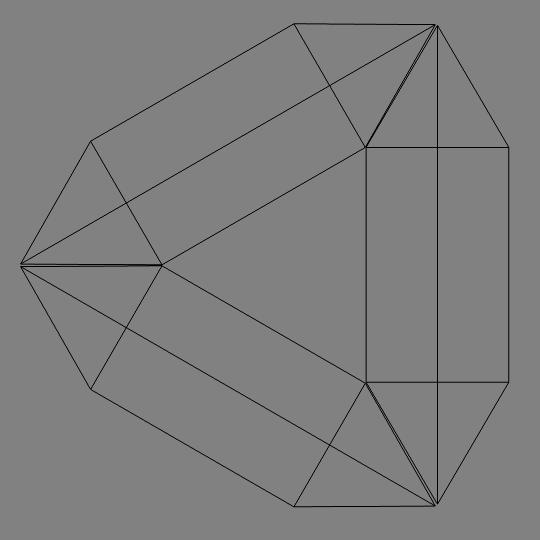
\includegraphics[width=4cm]{../Images/ballon3.png}
  \end{center}
\end{frame}

\begin{frame}{Vue d'ensemble}
 \begin{center}
		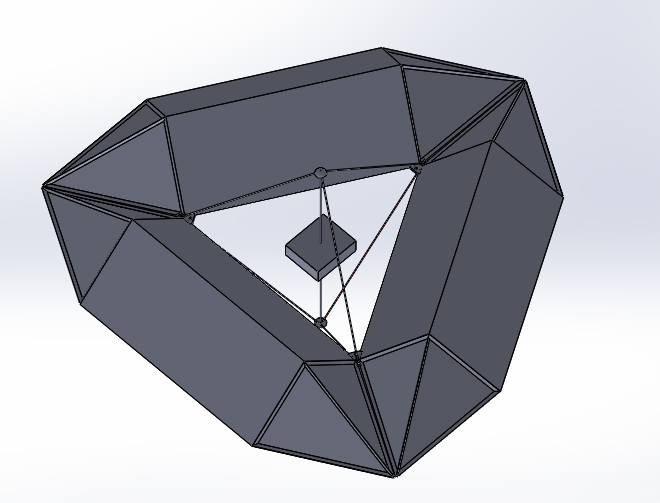
\includegraphics[width=10cm]{../Images/structure1_0.PNG}
 \end{center}
\end{frame}

\begin{frame}{Calcul des dimensions}
  Volume ballon~: volume de deux pyramides avec un parallélépipède~:
  \begin{center}
	\boxed{\displaystyle{V = 2(\frac{\sqrt{2 \times b^2}}{2} \times \tan \frac{\pi}{3} \times \frac{1}{3} \times b^2) + b^2}} \\
	$\displaystyle{V = \frac{\sqrt{6}}{3} \times b^3 + b^2 }$ \\
	$\displaystyle{b^3 \frac{\sqrt{6}}{3} + b^2 - 0.25 = 0}$
  \end{center}
  Où $b$ est la largeur du parallélépipède. \\
  Polynôme du troisième degré, résolution par bissection ou dichotomie.
\end{frame}

\begin{frame}[fragile]{Résolution par bissection}
  \begin{lstlisting}[frame=single]
etape = 1
largeur = 1
vol = volume(largeur)
cible = 0.25
epsilon = 1e-4
while abs(vol - cible) > epsilon:
	if vol < cible:
		largeur += etape
	else:
		largeur -= etape
	etape /= 2
	vol = volume(largeur)

print("volume = %f, diametre = %f" % (vol, largeur))
  \end{lstlisting}
\end{frame}

\begin{frame}{Patron du ballon}
  \begin{center}
    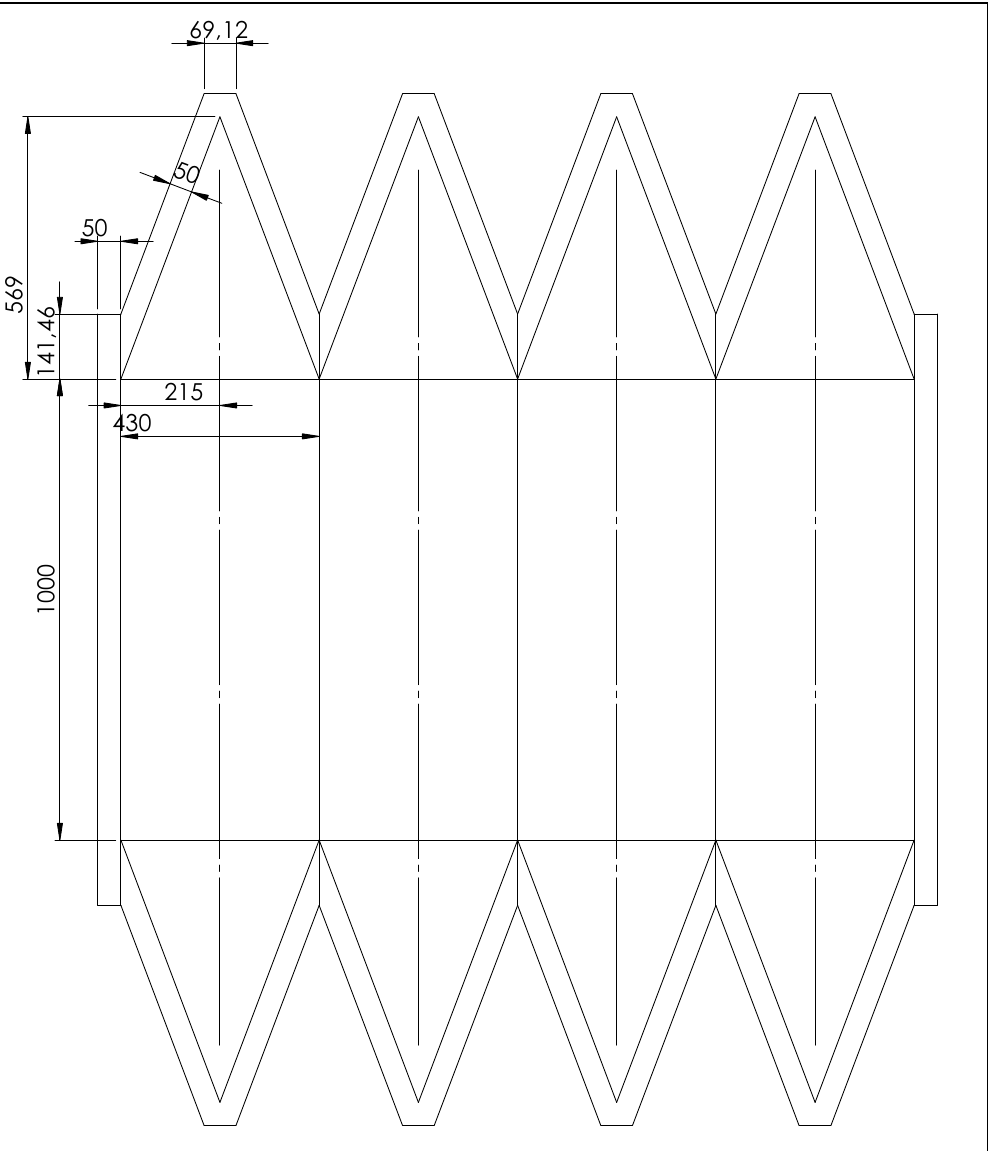
\includegraphics[width=6.5cm, angle=270]{../Images/plan_ballon.png}
  \end{center}
  Marge de 5cm pour le collage des coutures.
\end{frame}

\subsection{Enveloppe}

\begin{frame}{Liste des matériaux}
	\begin{tabular}{|l|p{0.35\linewidth}|p{0.35\linewidth}|}
		\hline
		Matériaux & Avantages & Inconvénients \\
		\hline

		\rowcolor{OrangeT}
		Latex &
		Facile à trouver dans le commerce &
		Seulement en forme sphérique~; peu étanche \\
		\hline

		\rowcolor{RedT}
		Hypalon & Étanche & Introuvable dans le commerce~; fragile aux ultraviolets \\
		\hline

		\rowcolor{GreenT}
		Mylar (PET) &
		Facile à trouver dans le commerce~; résistant à la traction~; peut être assemblé~; léger~: $17 g.m^{-2}$ &
		Raide~; fragile au cisaillement et à la perforation \\
		\hline

		\rowcolor{RedT}
		Chloroprène &
		& Introuvable dans le commerce \\
		\hline

		\rowcolor{RedT}
		Butyle &
		& Introuvable dans le commerce \\
		\hline
	\end{tabular}
\end{frame}

\subsection{Collage}

\begin{frame}{Liste des colles testées}
	\begin{tabular}{|p{0.3\linewidth}|p{0.3\linewidth}|p{0.3\linewidth}|}
		\hline
		Colle & Avantages & Inconvénients \\
		\hline

		\rowcolor{OrangeT}
		Néoprène (Polychloroprène) &
		Étanche, élastique, adhèrent &
		Difficile à appliquer \\
		\hline

		\rowcolor{OrangeT}
		406 (cyanoacrylate d'ethyle) et 770 (primaire) &
		Adhèrent, rigide, facile à appliquer &
		Fragile à l'eau \\
		\hline

		\rowcolor{GreenT}
		401 (cyanoacrylate d'ethyle) et 770 (primaire) &
		Très adhèrent, rigide, facile à appliquer &
		Fragile à l'eau \\
		\hline

		\rowcolor{RedT}
		330 et activateur &
		Élastique &
		Peu adhèrent \\
		\hline

		\rowcolor{RedT}
		Polyester &
		Polymérisation avec catalyseur &
		Peu adhèrent \\
		\hline
		
		\rowcolor{RedT}
		Polyuréthane &
		& Peu adhèrent \\
		\hline

		\rowcolor{RedT}
		Acétone &
		& Peu adhèrent \\
		\hline
		
		\rowcolor{RedT}
		Vinylique &
		Facile à appliquer &
		Peu adhèrent, temps de séchage trop long \\
		\hline

		\rowcolor{RedT}
		Acrylique &
		Facile à appliquer &
		Peu adhèrent \\
		\hline

	\end{tabular}
\end{frame}

\begin{frame}{Contrainte d'une colle}
  Différents types de contraintes sur une colle:
  \begin{center}
    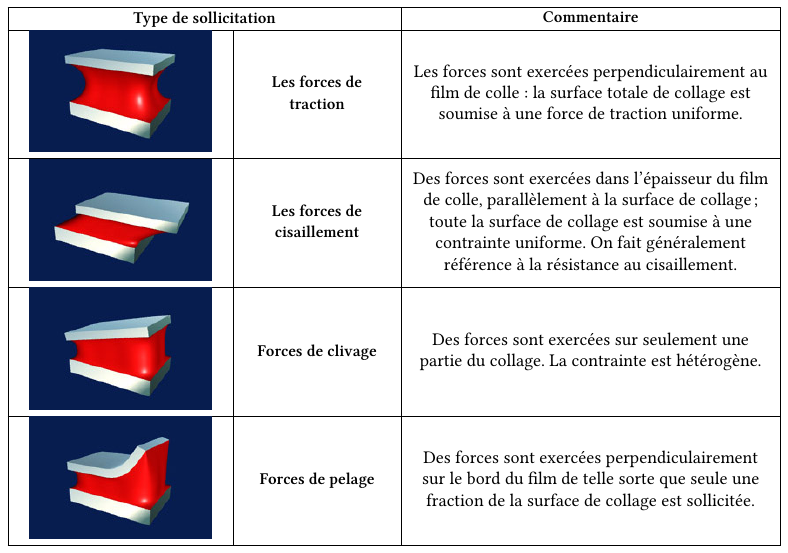
\includegraphics[width=10cm]{../Images/colle_contraintes.png}
  \end{center}
\end{frame}

\begin{frame}{Problème du collage}
  Collage du ballon extérieur~: contrainte de pelage, pire situation.
  \begin{figure}
    \centering
    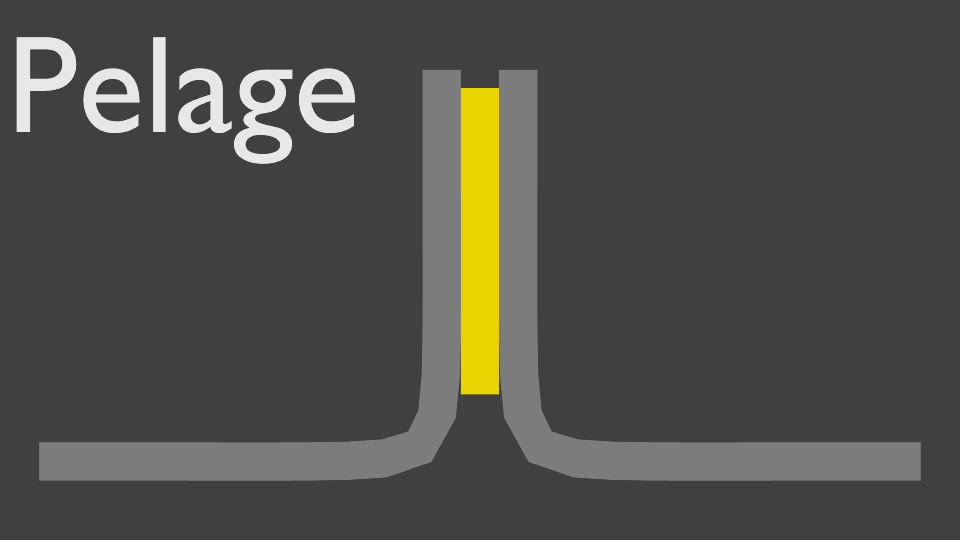
\includegraphics[width=5cm]{../Images/colle_pelage.png}
    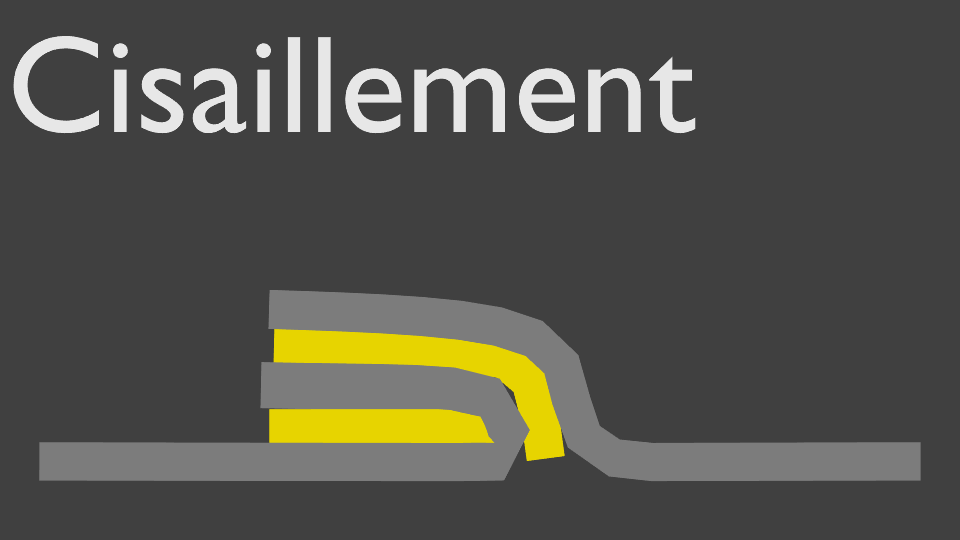
\includegraphics[width=5cm]{../Images/colle_cisaillement.png}
    \caption{À gauche collage favorisant une contrainte de pelage, à droite collage favorisant une contrainte de cisaillement}
  \end{figure}
  Solution~: coller la couture sur le ballon.
\end{frame}

\begin{frame}{Tests traction 401 (cyanoacrylate)}
  \begin{figure}[!t]
    \centering
    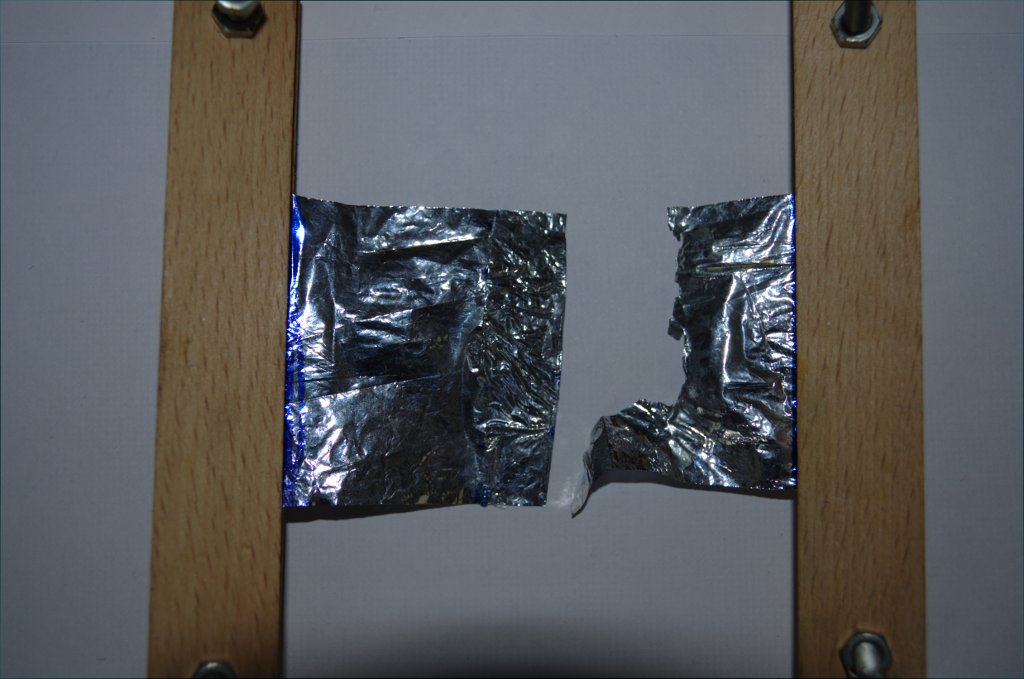
\includegraphics[width=4.5cm]{../Images/test_cisaillement.png}
    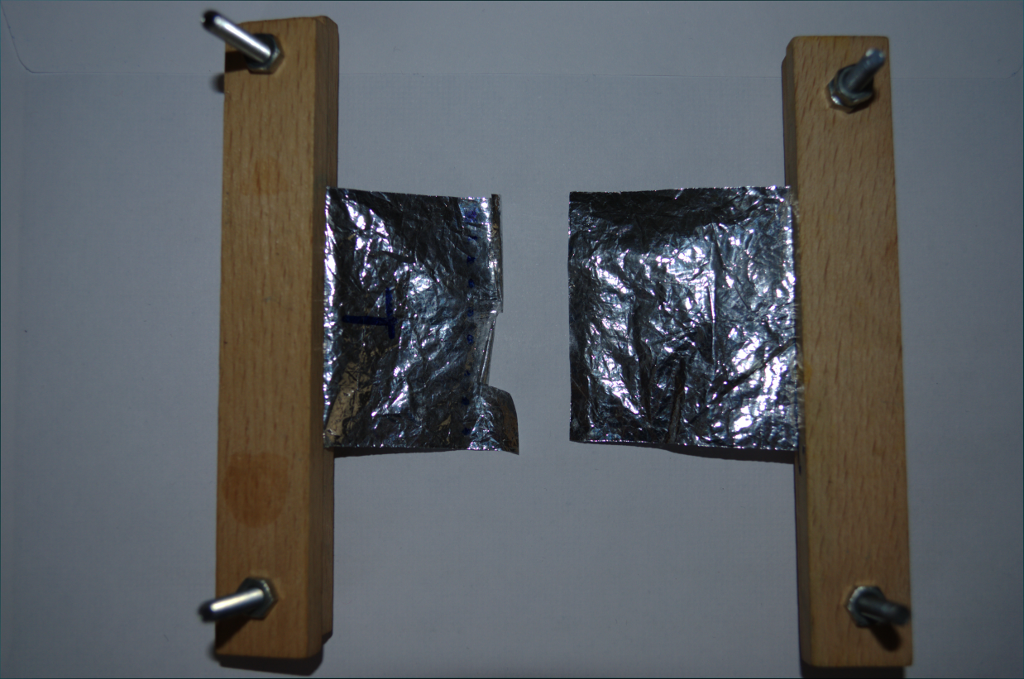
\includegraphics[width=4.5cm]{../Images/test_pelage.png}
    
    \caption{À gauche~: test de cisaillement, rupture du substrat. À droite~: test de pelage, rupture du collage}
  \end{figure}
  Résultats des tests de traction~:
  \begin{center}
    \begin{tabular}{|c|c|}
      \hline
      Pelage & Cisaillement \\
      \hline
      $0.45 N.cm^{-2}$ & $12.1 N.cm^{-2}$ \\
      \hline
    \end{tabular}
  \end{center}
  Augmentation de la résistance de $\times 27$.
\end{frame}


\subsection{Étanchéité}
\begin{frame}{Protocole de test d'étanchéité}
 Étanchéité du PET et des collages. Détection des fuites avec de l'eau savonneuse. Colle acrylique pour boucher les fuites.

\begin{figure}[H]
	\centering
	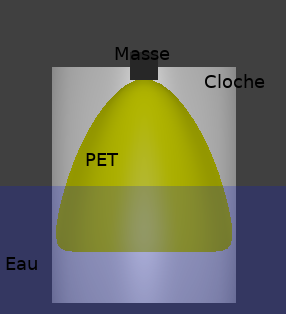
\includegraphics[width=4.5cm]{../Images/etancheite.png}
	\caption{Test d'étanchéité du PET, le PET est maintenu par la cloche dans l'eau, nous mesurons la chute de la masse disposée au dessus du PET.}
\end{figure}

\end{frame}

\begin{frame}{Tests d'étanchéité}

\begin{center}
    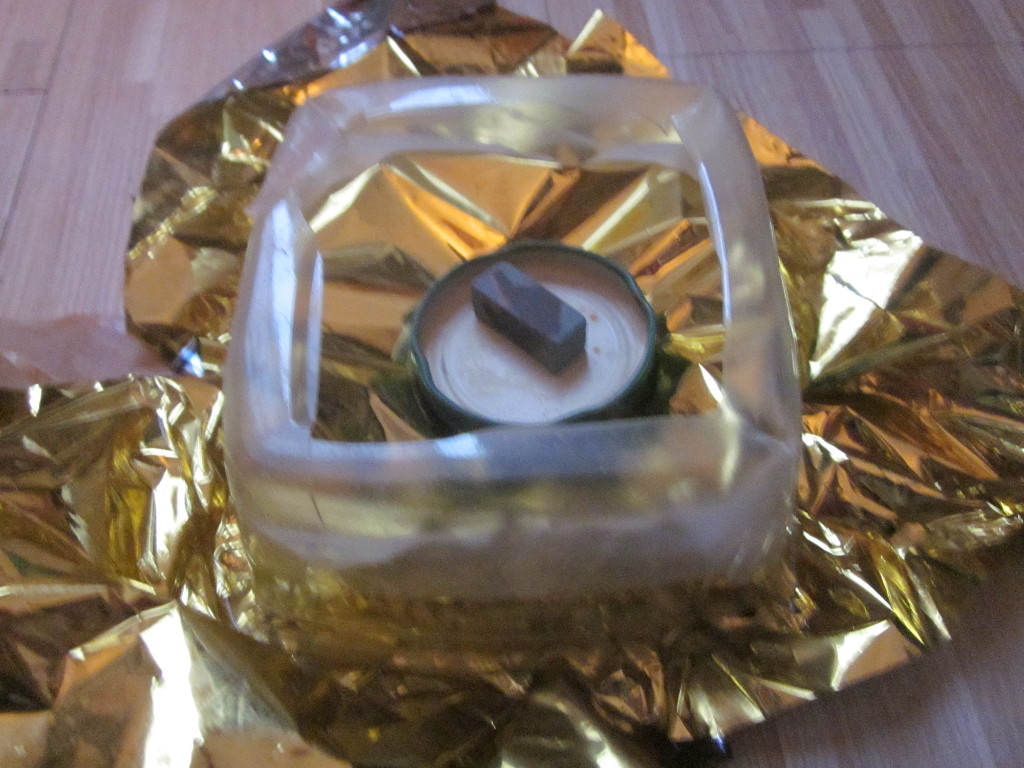
\includegraphics[width=3.5cm]{../Images/cloche_pet.JPG}
    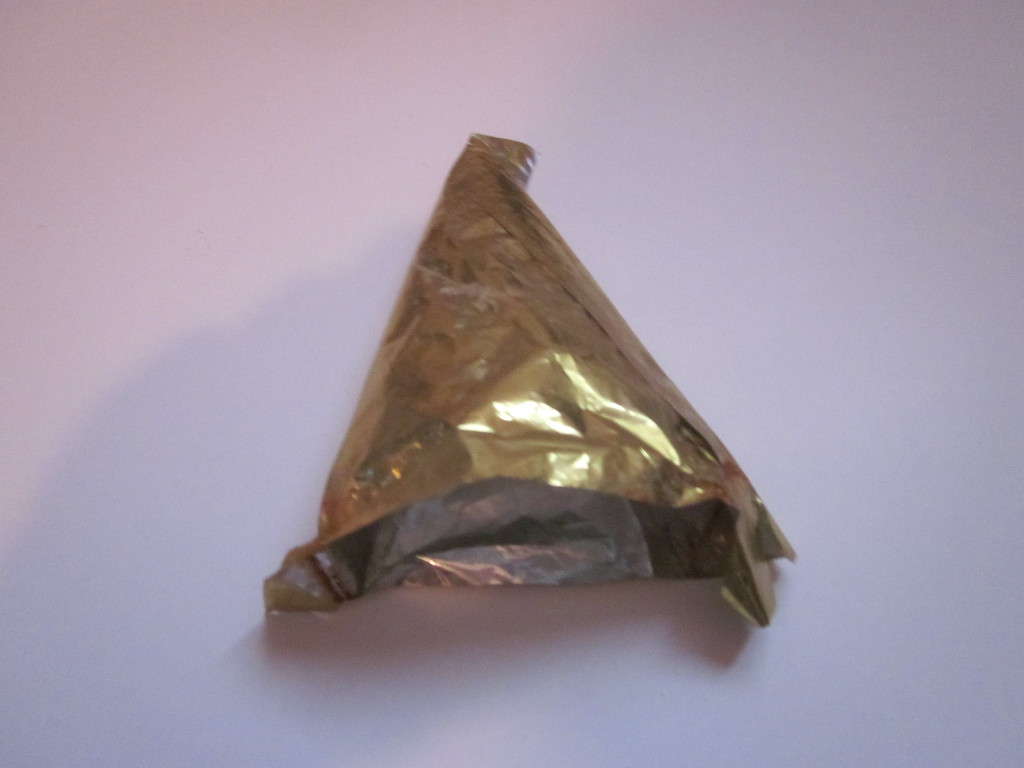
\includegraphics[width=3.5cm]{../Images/cloche_colle.JPG}
\end{center}

\begin{center}
    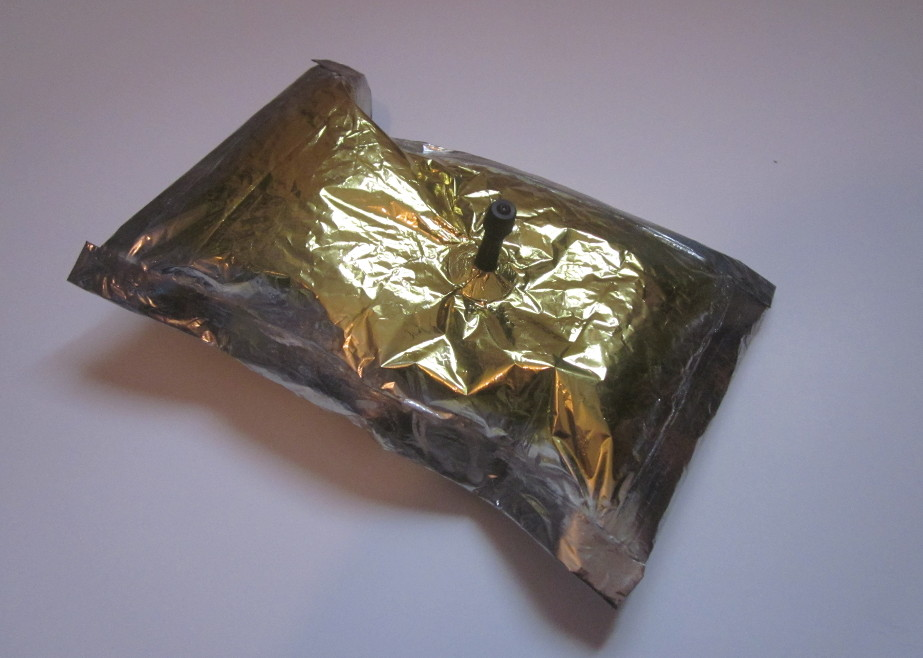
\includegraphics[width=4cm]{../Images/ballon_etanche.JPG}
    \captionof{figure}{Ballon de test d'étanchéité.}
\end{center}

Présence de fuites non détectables.

\end{frame}


\subsection{Assemblage ballon}

\begin{frame}{Assemblage des ballons}
  \begin{center}
	\begin{tabular}{cc}
		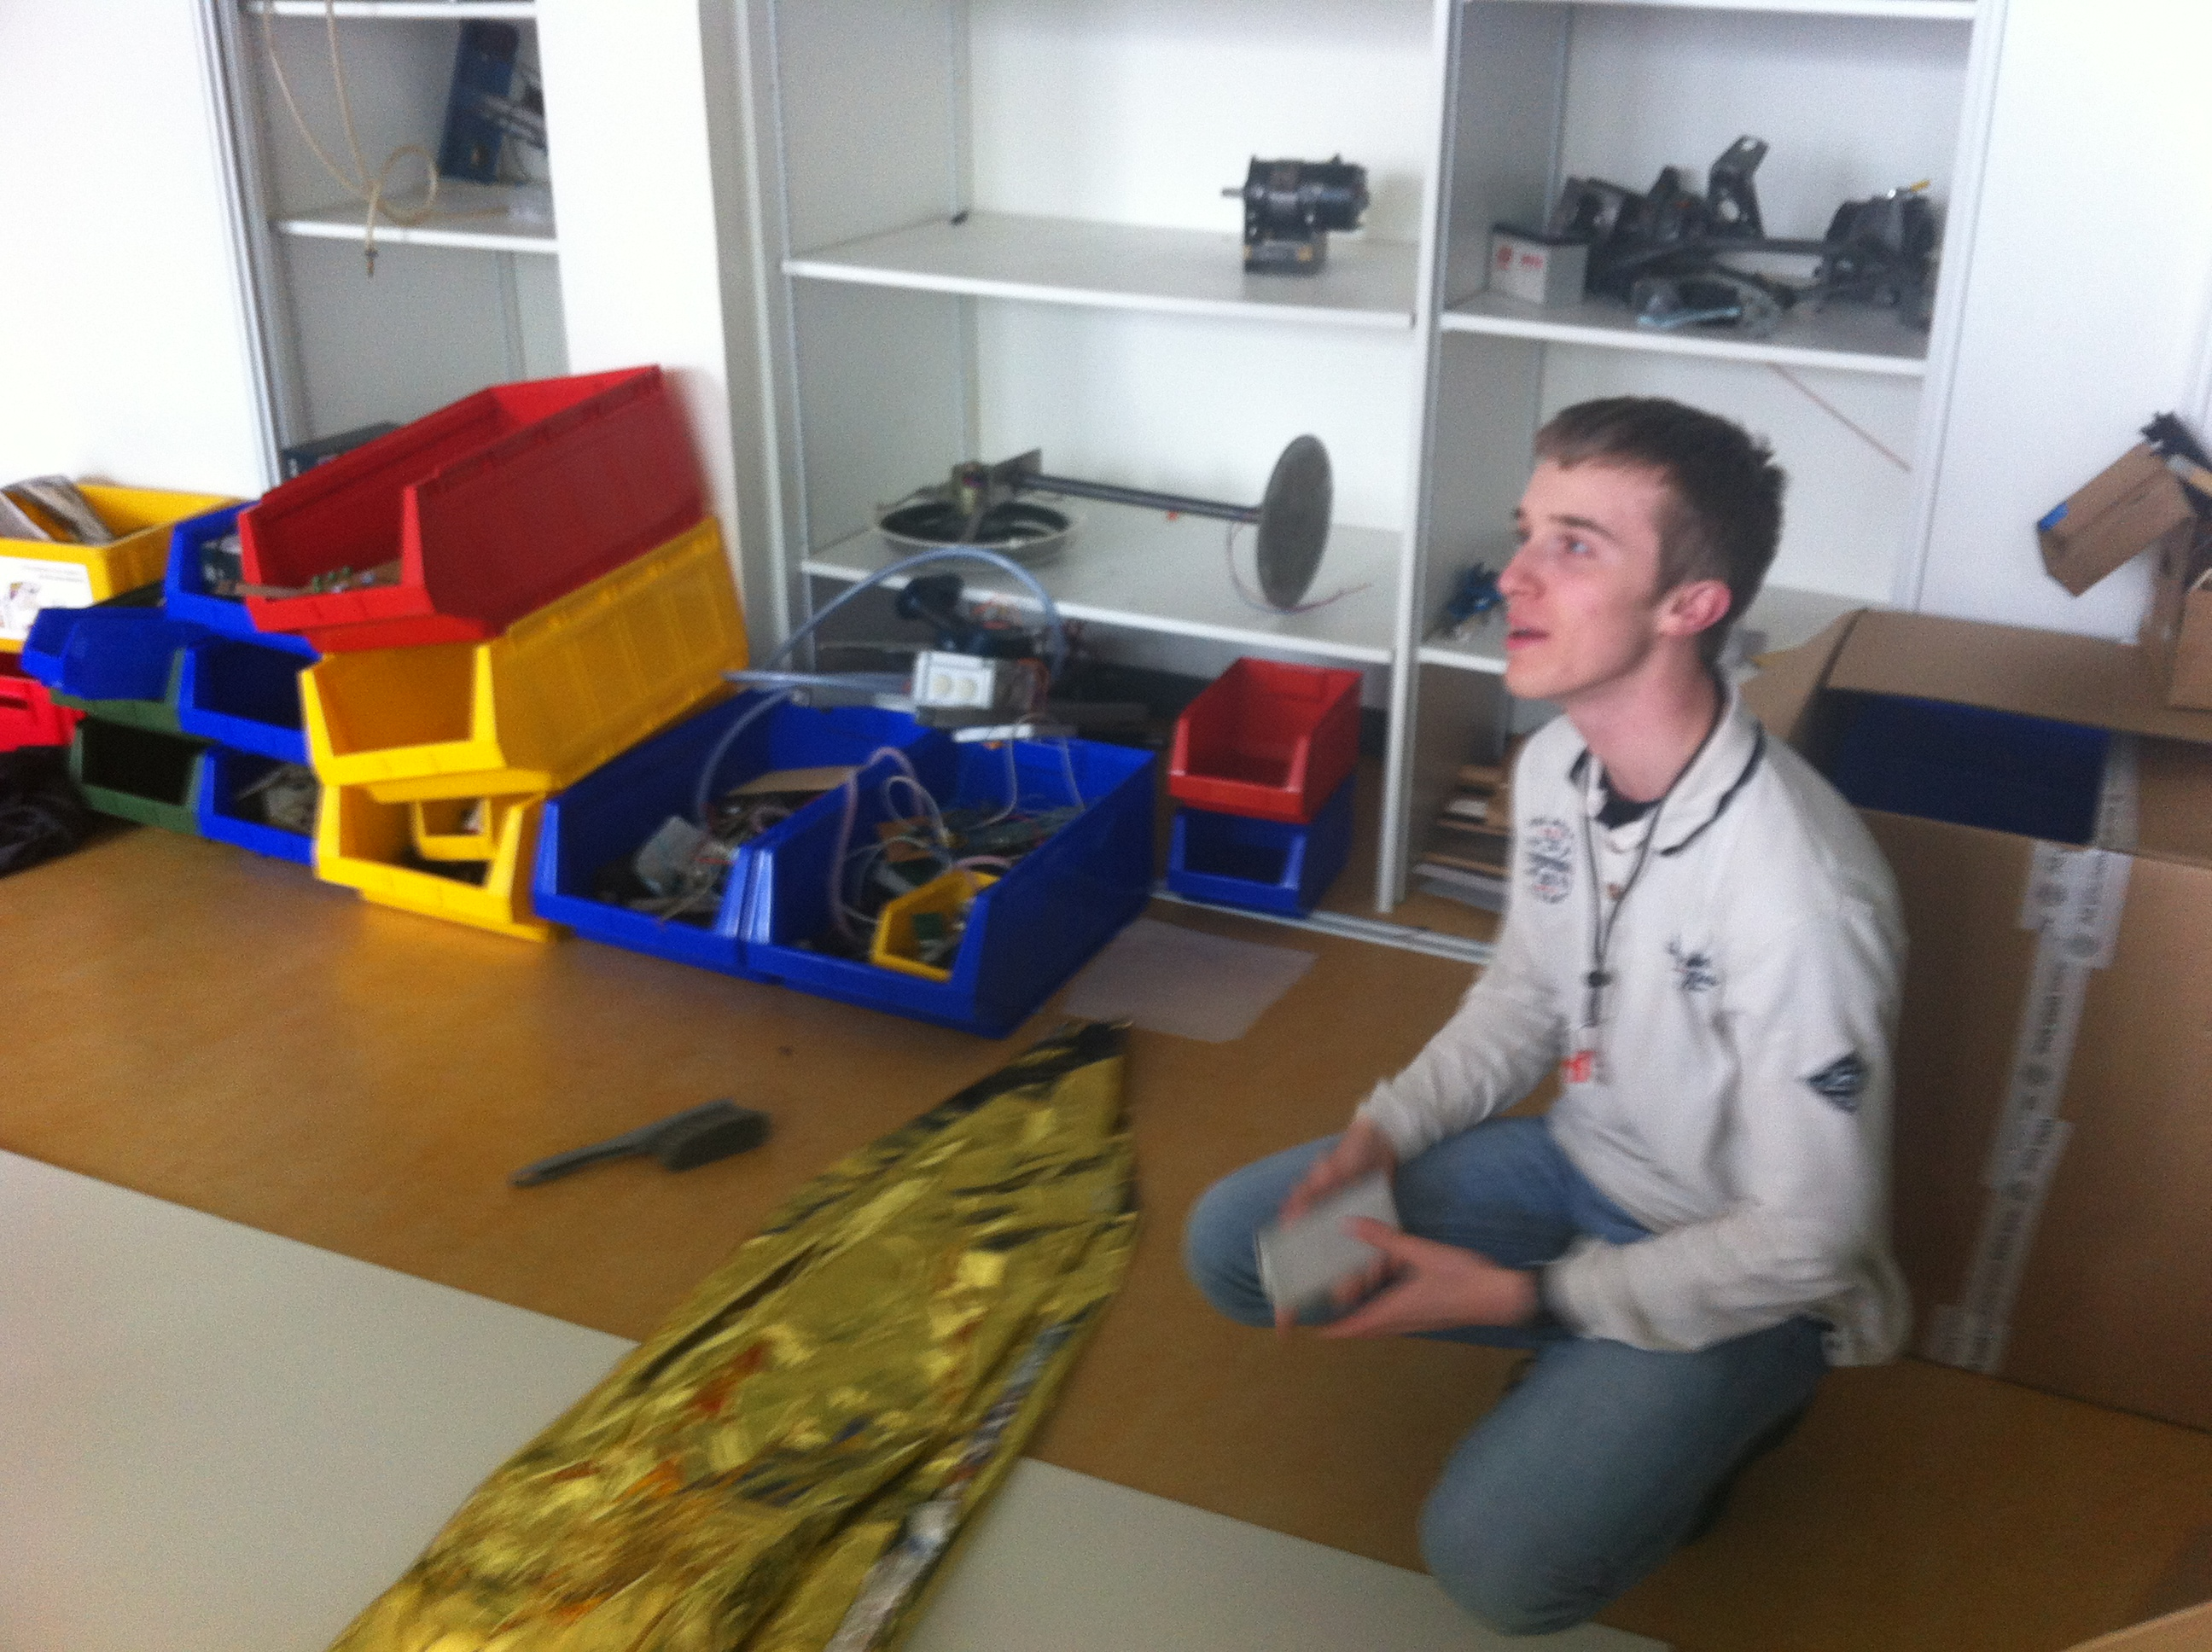
\includegraphics[width=4.5cm]{../Images/assen_0.JPG} &
		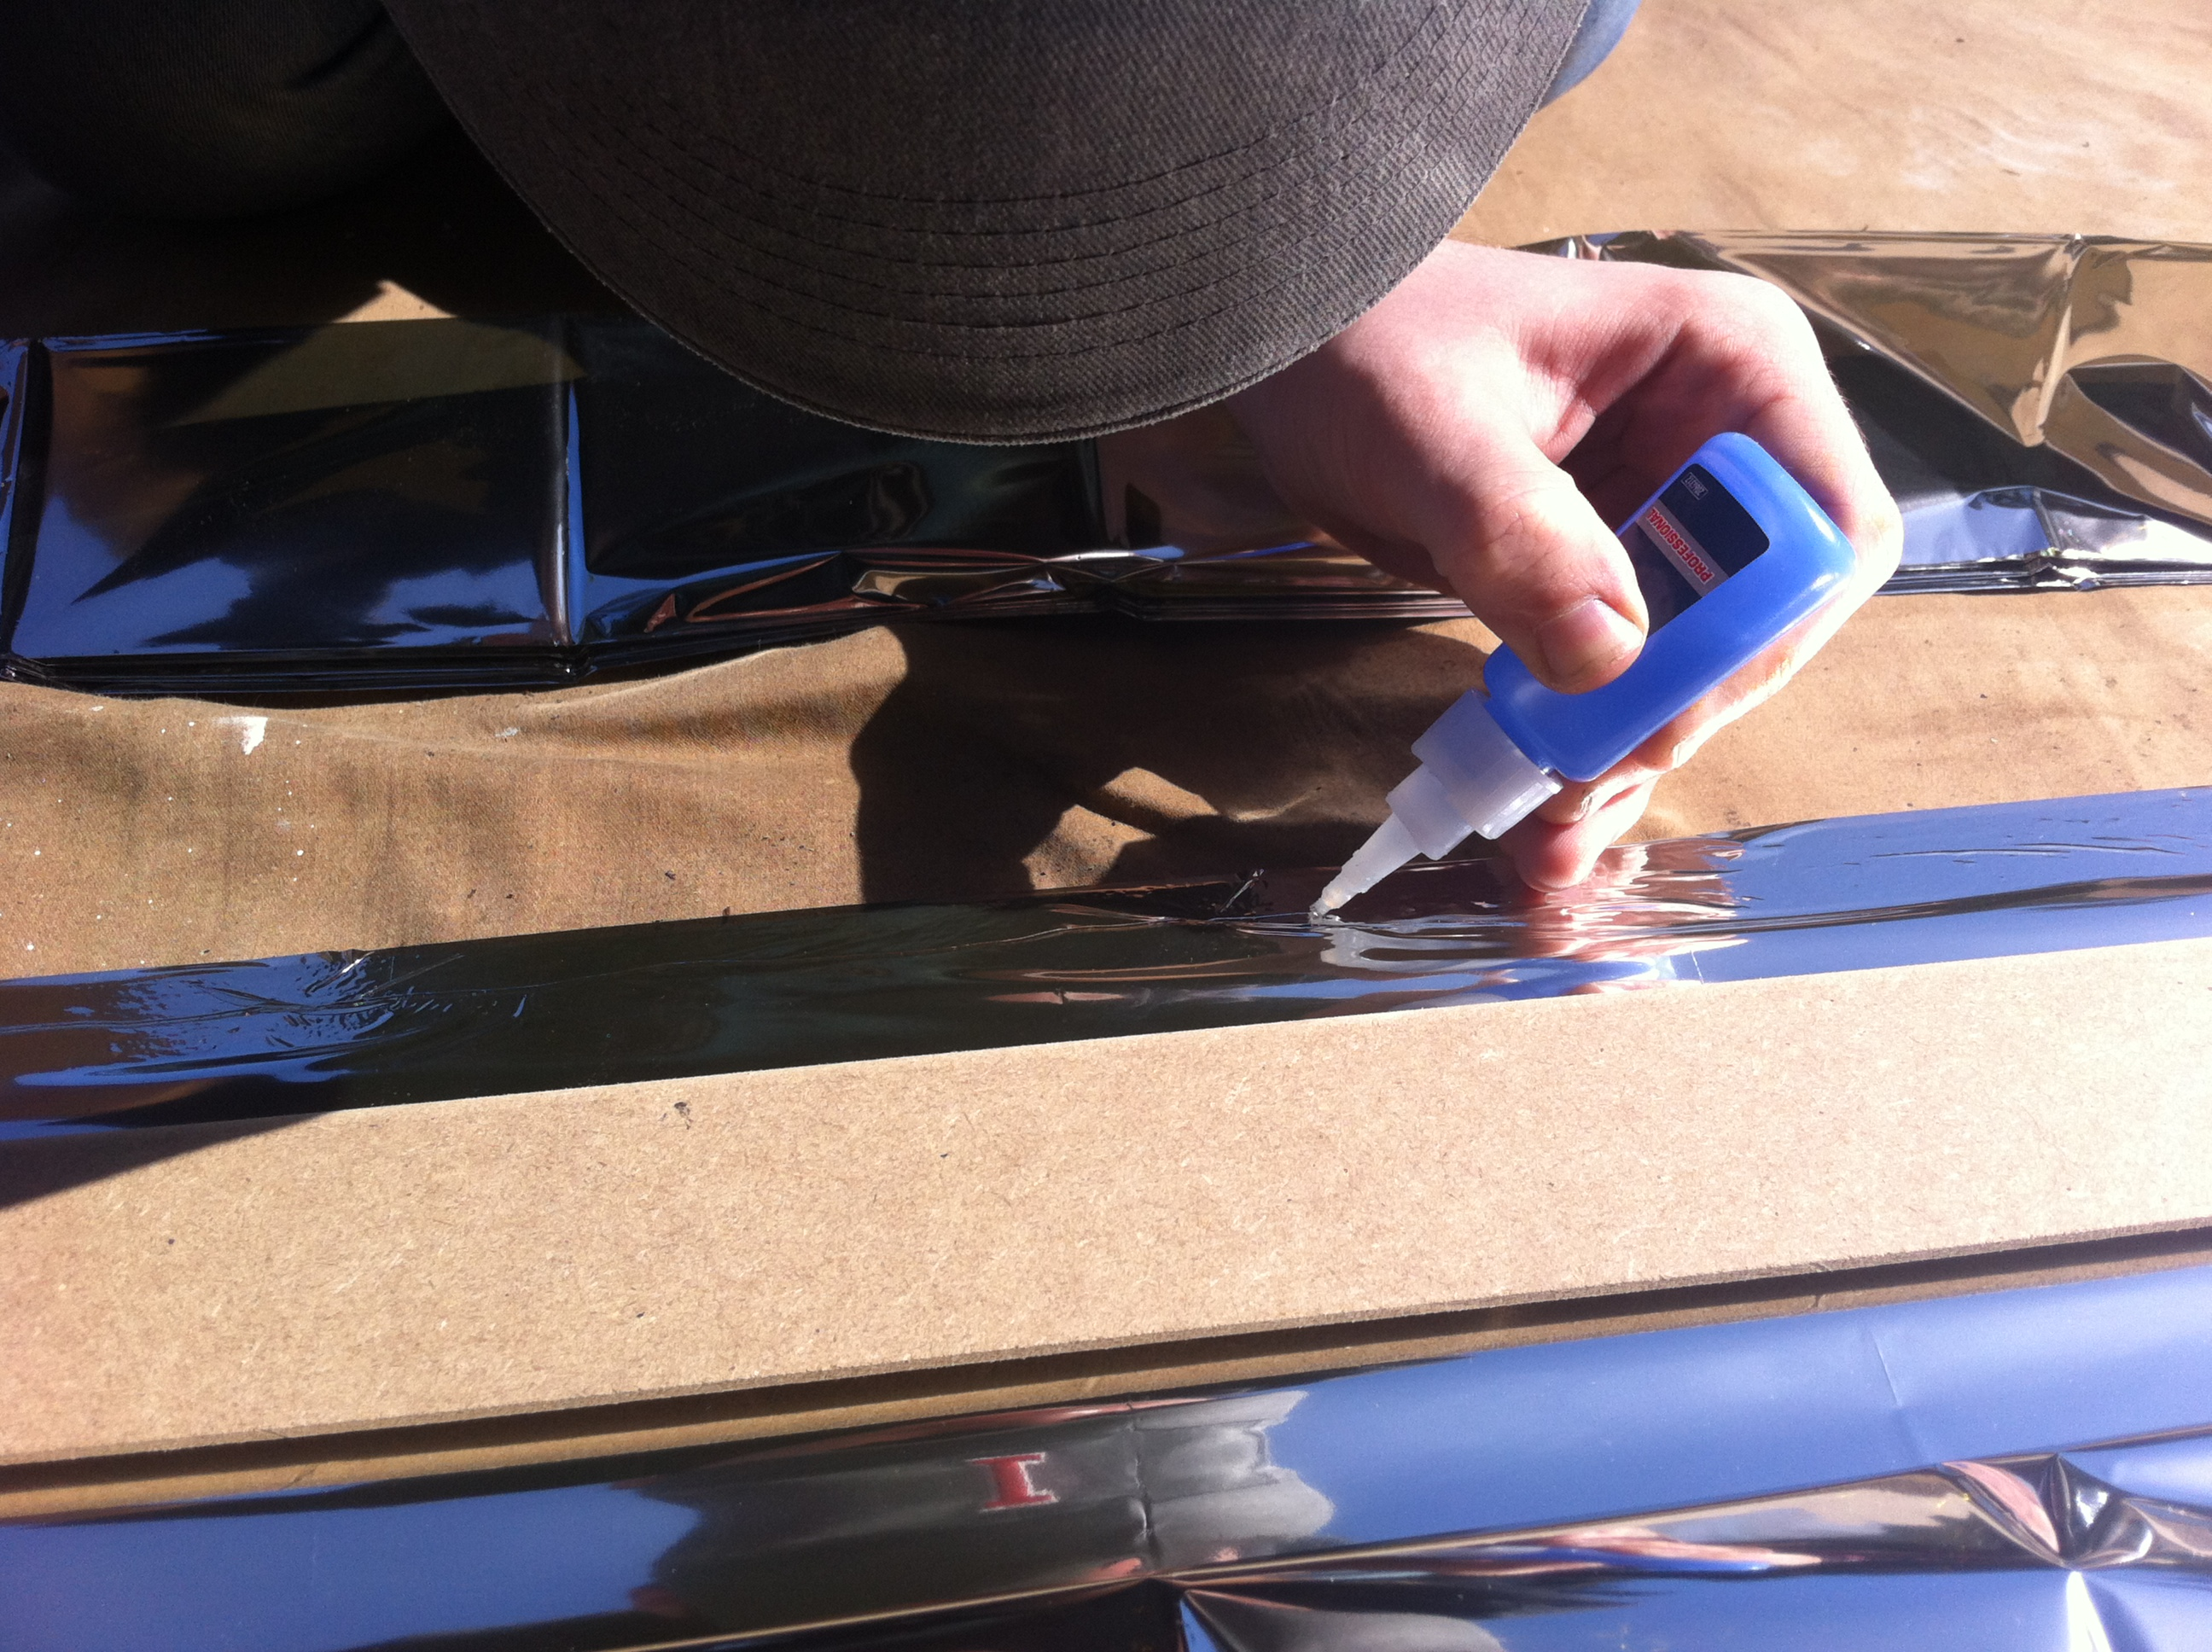
\includegraphics[width=4.5cm]{../Images/assen_1.JPG} \\
		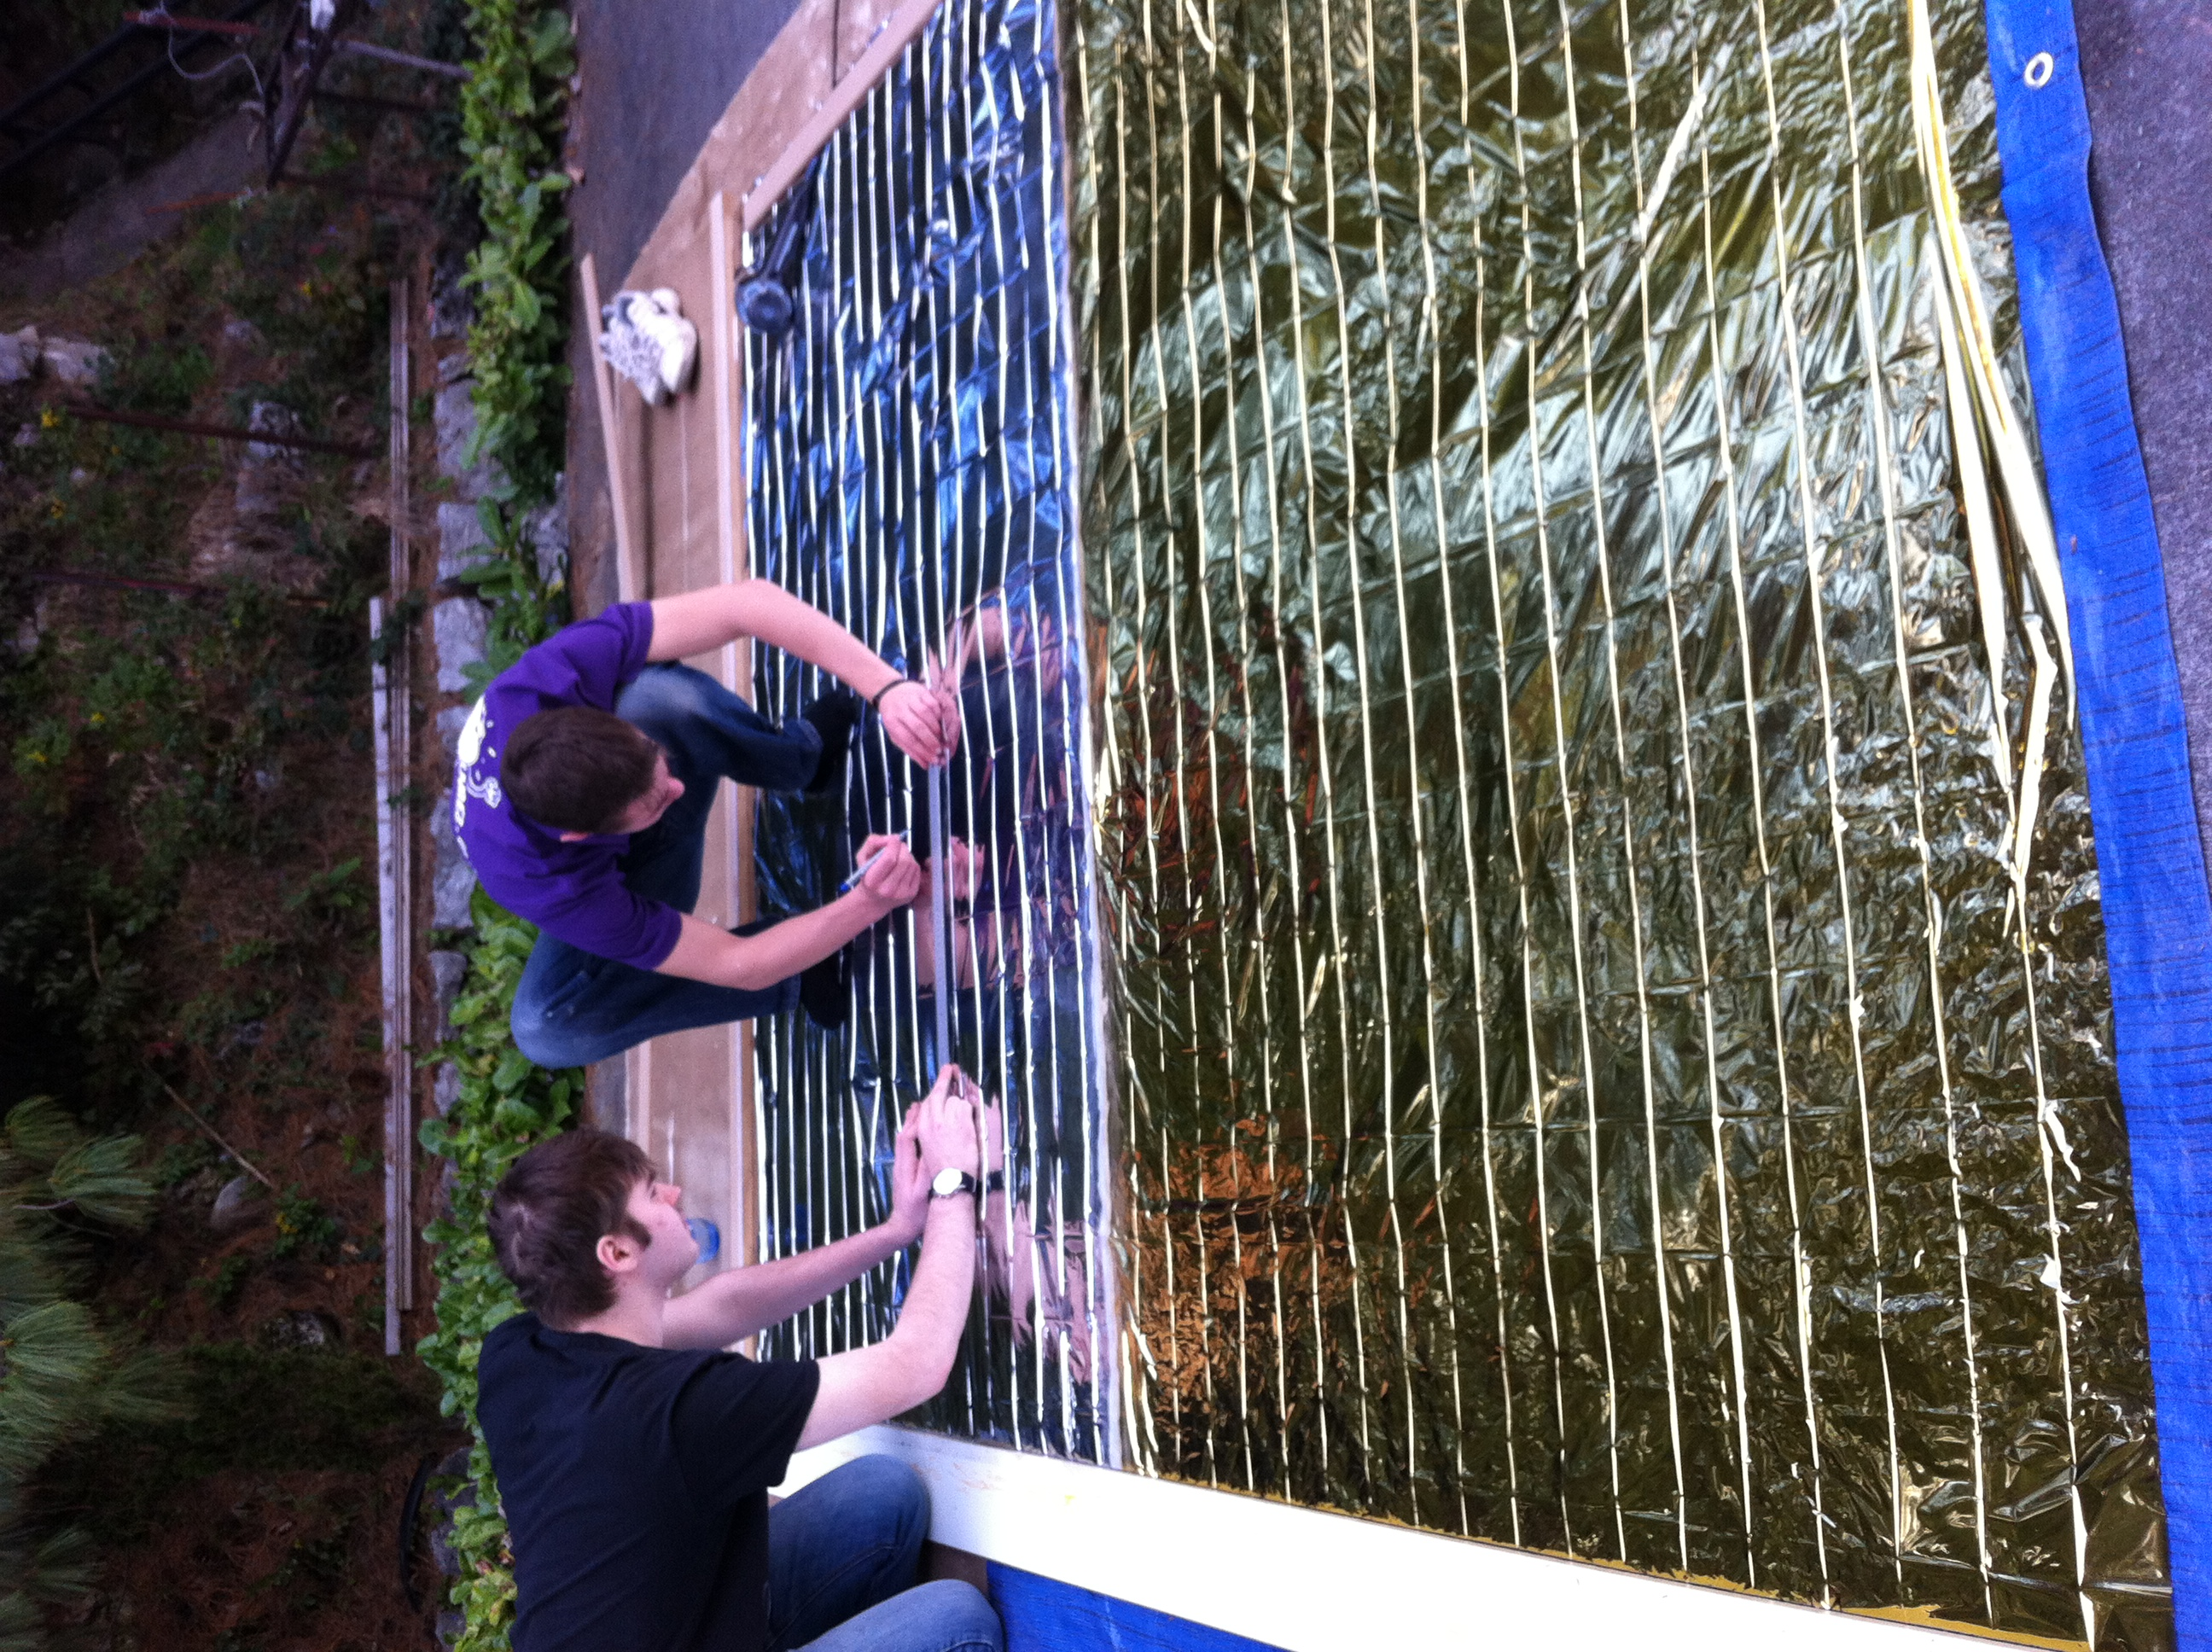
\includegraphics[width=3cm]{../Images/assen_2.JPG} &
		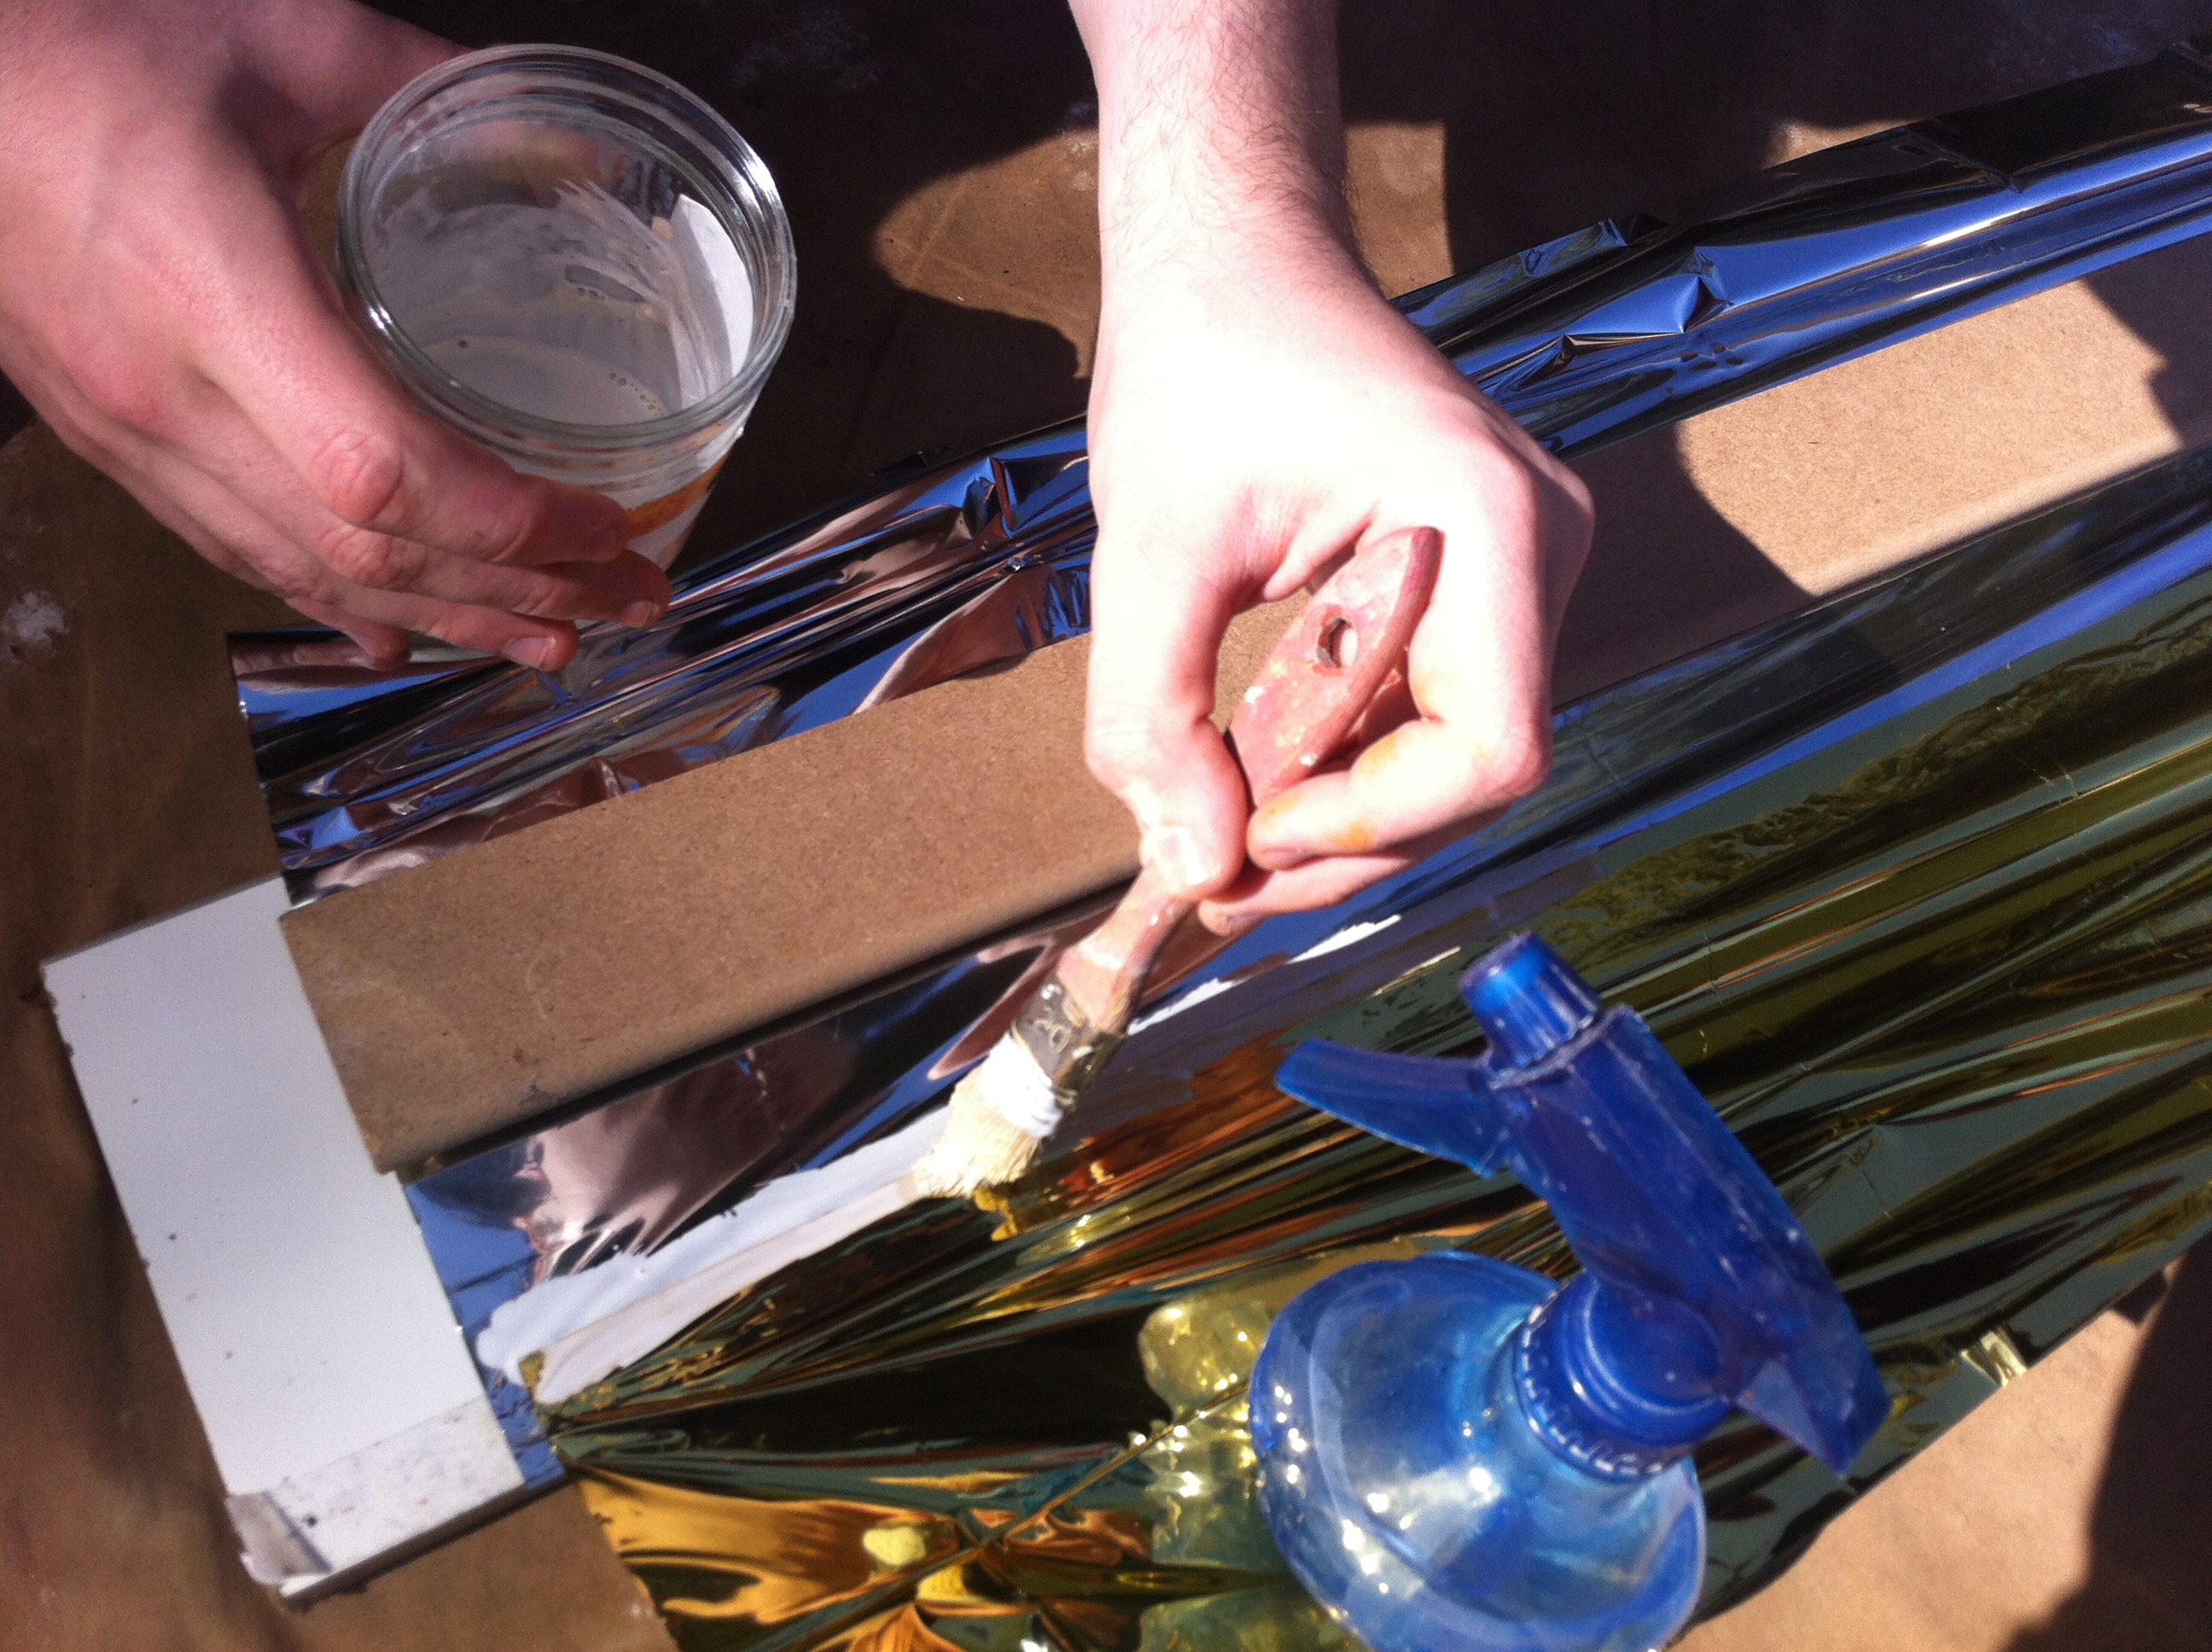
\includegraphics[width=4.5cm]{../Images/assen_3.JPG} \\
	\end{tabular}
  \end{center}
\end{frame}


\end{document}